\documentclass[../main.tex]{subfiles}
\begin{document}
\clearpage
\section{Свойства множеств достижимости нелинейных систем с интегральными ограничениями на малых интервалах времени}
    В этом разделе будут описаны результаты, на которые опираются дальнейшие исследования. 
	В первом параграфе описывается условие выпуклости нелинейного отображения малого шара в гильбертовом пространстве, полученное  Б.Т. Поляком\cite{Polyak2001}.
	Во втором параграфе описывается применение этого условия для обоснования выпуклости множеств достижимости нелинейных систем при ограничении на управление, заданном шаром достаточно малого радиуса.
	В третьем параграфе исследуются условия, при которых множества достижимости нелинейных систем с интегральными ограничениями оказываются выпуклыми на малых интервалах времени. 
    
    \subsection{Выпуклость отображения малого шара.}
    
    Пусть $X$, $Y$ --- гильбертовы пространства, а $f: X \rightarrow Y$ --- нелинейное отображение с липшицевой производной, определенное  на шаре $B_X(a,r) = \{x \in X: \| x - a\| \leqslant r\}$, тогда 
    \begin{gather}\label{lip_cond}
        \| f'(x) - f'(z) \| \leqslant L \| x - z \|, \quad \forall x,z \in B_X(a,r).
    \end{gather}
    Предположим, что $a$ --- регулярная точка отображения $f$, то есть линейный оператор $f'(a)$ отображает $X$ на $Y$ и тогда найдется $\nu > 0$, такое что
    \begin{gather}\label{regularity_cond}
        \| f'(a)^*y\| \geqslant \nu \| y\|, \quad \forall y \in Y.
    \end{gather}
    Например, если множества $X,Y$ --- конечномерные, $X\in\mathbb{R}^n$, $Y\in\mathbb{R}^m$, то условие \eqref{regularity_cond} выполняется, если $ \operatorname{rank} f'(a) = m$. В этом случае $\nu$ --- наименьшее сингулярное число $f'(a)$. 
    \begin{theorem}\label{PolyakTh}
        Если выполняются \eqref{lip_cond}, \eqref{regularity_cond}  и 
        \begin{gather}
            \varepsilon < \min\left\{r,\frac{\nu}{2L}\right\},
        \end{gather}
        тогда образ шара $B_X(a,\varepsilon) = \{x \in X: \| x - a\| \leqslant \varepsilon\}$ при отображении $f$ выпуклый, то есть $F = 
        \{f(x): x \in B_X(a,\varepsilon)\}$ --- выпуклое множество в $Y$. Более того, это множество сильно выпуклое и его граница состоит из образов граничных точек шара: $\partial F \subset f(\partial B_X(a,\varepsilon))$
    \end{theorem}
    
    \subsection{Выпуклость множеств достижимости нелинейных систем с интегральными ограничениями}
    На интервале времени $ t_0 \leqslant t \leqslant \overline{T} $ рассмотрим нелинейную систему, аффинную по управлению
	\begin{gather}\label{nonlinear}
		\begin{gathered}
			\dot{x}(t)=f_1(t,x(t))+f_2(t,x(t))u(t), \qquad x(t_0) = x_0.
		\end{gathered}
	\end{gather}
	Здесь $ x \in \mathbb{R}^n $ -- вектор состояния, $ u \in \mathbb{R}^r $ -- управление,  $ \overline{T} $ --- некоторое фиксированное положительное число.
	
	
	Функции $ f_1: \mathbb{R}^{n+1} \rightarrow \mathbb{R}^{n} $, $ f_2: \mathbb{R}^{n+1} \rightarrow \mathbb{R}^{n \times r} $ предполагаются непрерывными и непрерывно-дифференциру-\\емыми по $ x $.
	Также предполагается, что функции $ f_1 $, $ f_2 $ удовлетворяют условиям
	\begin{gather*}
		\begin{gathered}
			\left\| f_1(t,x) \right\| \leqslant	l_1(t)(1 + \left\| x \right\| ), \\
			\left\| f_2(t,x) \right\| \leqslant	l_2(t),  \qquad t_0 \leqslant t \leqslant \overline{T}, \qquad   x \in \mathbb{R}^n,
		\end{gathered}
	\end{gather*}
	где $ l_1(\cdot) \in \mathbb{L}_1[t_0,\overline{T}] $, $ l_2(\cdot) \in \mathbb{L}_2[t_0,\overline{T}] $.
	
	Под $ \mathbb{L}_1[t_0,\overline{T}],  \mathbb{L}_2[t_0,\overline{T}]  $ будем понимать,  соответственно, пространства
	интегрируемых и интегрируемых с квадратом скалярных или вектор-функций  на $ [t_0,\overline{T}] $. Управление $u(t)$ будем выбирать из
	пространства $\mathbb{L}_2[t_0,\overline{T}]$ вектор-функций,  скалярное произведение в котором определено равенством
	\begin{gather*}
		\left(u(\cdot),\upsilon(\cdot) \right) = \int_{t_0}^{\overline{T}}u^{\top}(t)\upsilon(t) \, dt.
	\end{gather*}
	Управление $ u(\cdot) $ ограничим шаром радиуса $ \mu, \mu > 0 $
	\begin{gather}\label{constr}
		\lVert u(\cdot)\rVert^2_{\mathbb{L}_2} = \left(u(\cdot),u(\cdot) \right) \leqslant \mu^2.
	\end{gather}
	
	В условиях описанных предположений, каждому $ u(\cdot) \in \mathbb{L}_2 $ соответствует единственное абсолютно непрерывное решение $ x(t)=x(t,u(\cdot)) $ системы \eqref{nonlinear}, определённое на интервале $ [t_0,\overline{T}] $.
	
	Все траектории $ x(t) $ системы \eqref{nonlinear}, отвечающие удовлетворяющим \eqref{constr} управлениям,  лежат внутри некоторого компактного множества $ D \subset \mathbb{R}^n $.
	
	Дадим здесь несколько определений, которыми будем пользоваться в дальнейшем.
	
	Пусть $ 0 <  T \leqslant \overline{T} $.
	\begin{definition}
		{\textit  Множеством достижимости} $ G(T,\mu) $ системы \eqref{nonlinear} в пространстве состояний в момент времени $ T $ назовем множество всех концов траекторий $ x(T) \in \mathbb{R}^n $,  которые могут быть порождены управлениями	$ u(t) \in B_{\mathbb{L}_2}(0,\mu) =\left\lbrace u:\lVert u(\cdot)\rVert^2_{\mathbb{L}_2} \leqslant \mu^2\right\rbrace  $,
		\begin{gather*}
			G(T,\mu)=\{x\in \mathbb{R}^n:\exists u(\cdot)\in B_{\mathbb{L}_2}(0,\mu),\; x=x(T,x^0,u(\cdot))\}.
		\end{gather*}
	\end{definition}
	\begin{definition}
		Пусть $ x(t,x_0,u(\cdot)) $ --- движение, отвечающее управлению $ u(\cdot)$. Тогда назовем систему
		\begin{gather}\label{linear}
			\delta \dot{x} =  A(t) \delta x + B(t) \delta u, \qquad t_0 \leqslant t \leqslant T, \qquad \delta x(t_0) = 0,
		\end{gather}
		{\textit линеаризацией} системы \eqref{nonlinear} вдоль траектории $ x(t,x_0,u(\cdot)) $, если 
		\begin{gather*}
		    A(t) = \dfrac{\partial f_1}{\partial x} (t,x(t,x_0,u(\cdot))) + \dfrac{\partial f_2}{\partial x}(t,x(t,x_0,u(\cdot))) u(\cdot), \  B(t) = f_2 (t,x(t,0)).
		\end{gather*} Здесь $ A(t) $ представляет собой матрицу Якоби функции $ f_1 + f_2 u(\cdot) $, вычисленную вдоль траектории $ x(t,u(\cdot)) $.
	\end{definition}
	\begin{definition}
	Симметричная матрица, определённая равенством
		\begin{gather*}
			W(T) = \int_{t_0}^{T}X(T,t)B(t)B^{\top}(t)X^{\top}(T,t) \, dt,
		\end{gather*}
	называется грамианом управляемости системы \eqref{linear} на интервале времени $  t_0 \leqslant t \leqslant T $.
	\end{definition}
	Здесь $ X(\tau_1,\tau_0)= \Phi(\tau_1) \Phi^{-1}(\tau_0) $, где $\Phi(t) $ --- фундаментальная матрица решений однородной системы, удовлетворяющая уравнению 
	\begin{gather*}
		\dot{\Phi}(t) = A(t) \Phi(t), \qquad \Phi(t_0) = I.
	\end{gather*}

	Система \eqref{linear} вполне управляема на  $ [t_0, T] $ тогда и только тогда, когда ее грамиан управляемости $W(T)$ --- положительно определенная матрица.
	
	При фиксированном $x_0$ введем отображение $F: \mathbb{L}_2[0,T] \rightarrow \mathbb{R}^n $ равенством $Fu(\cdot) = x(T,u(\cdot))$: здесь $ x(T,u(\cdot))$ --- решение системы \eqref{nonlinear}, порожденное управлением $u(\cdot)$. 
	
	Это отображение имеет непрерывную производную Фреше, определяемую равенством $ F'(u(\cdot))\delta u(\cdot) = \\=\delta x(T)$, где $\delta x(T)$ --- решение линеаризованной вдоль пары $\left( x(t,u(\cdot)),u(\cdot)\right)  $ системы \eqref{linear}, порожденное управлением $\delta u(\cdot)$ при нулевых начальных условиях.
	
	 Тогда, управляемость системы \eqref{linear} означает регулярность отображения $F$ при $u = 0$, а множество достижимости $G(T,\mu)$ есть образ гильбертова шара $B_{\mathbb{L}_2}(0,\mu)$ при его отображении $F$.
	
	Применяя теорему \ref{PolyakTh} к отображению $F$, получим, что в условиях описанных преположений относительно функций $f_1$ и $f_2$, множество достижимости $G$ выпукло при достаточно малых $\mu > 0$.
	
    \subsubsection{Выпуклость множеств достижимости на малых интервалах времени}
    Рассмотрим здесь нелинейную систему \eqref{nonlinear} на малом интервале времени $\ t_0 \leqslant t \leqslant t_0 + \overline{\varepsilon} $.
    \begin{gather}\label{nonlinearT}
			\dot{x}(t)=f_1(t,x(t))+f_2(t,x(t))u(t), \qquad x(t_0) = x_0.
	\end{gather}
    Здесь $ \overline{\varepsilon} $ --- некоторое фиксированное положительное число, а кроме принятых в предыдущем разделе допущений относительно функций $f_1$ и $f_2$, которые предполагаются справедливыми на интервале $t_0 \leqslant t \leqslant t_0 + \overline{\varepsilon} $ введем следующее.
    \begin{assumption}\label{Pred}
    	Функции $f_1(t,x)$ и $f_2(t,x)$ имеют непрерывные производные по $x$, которые удовлетворяют условию Липшица при всех $t \in [t_0;t_0+\varepsilon]$,$x_1, x_2 \in D$.
    	\begin{gather*}
    			\left\| \frac{\partial f_1}{\partial x}(t,x_1) - \frac{\partial f_1}{\partial x}(t,x_2) \right\| \leqslant L_3 \| x_1 - x_2\|, \quad 	\left\| \frac{\partial f_2}{\partial x}(t,x_1) - \frac{\partial f_2}{\partial x}(t,x_2) \right\| \leqslant L_4 \| x_1 - x_2\|,
    	\end{gather*}
    	где $L_i \geqslant 0$ для $i = 3,4$.
    \end{assumption}

     Управление $u(\cdot)$ будем выбирать из
    пространства интегрируемых с квадратом функций $\mathbb{L}_2[t_0,t_0+\bar{\varepsilon}]$ и ограничим шаром радиуса $ \mu > 0 $ в этом пространстве
    \begin{gather*}
    	\lVert u(\cdot)\rVert^2_{\mathbb{L}_2} = \left(u(\cdot),u(\cdot) \right) \leqslant \mu^2.
    \end{gather*}
	Пусть $ 0 <  \varepsilon \leqslant \bar{\varepsilon} $.  
	
	Далее, используя замену времени, мы сведем задачу описания множества достижимости на малом интервале к аналогичной задаче на фиксированном интервале для системы, уравнения которой и интегральные ограничения на управления зависят от малого параметра.
    Произведя замену времени
    $ t = \varepsilon \tau + t_0 $ и приняв обозначения $ z(\tau) = x(\varepsilon \tau + t_0) $ и $ \upsilon(\tau) = \varepsilon u(\varepsilon \tau + t_0) $  получим из \eqref{nonlinearT}
        \begin{equation}\label{epsnonlinear}
    	\dot{z}(\tau)=\widetilde{f}_1(\tau,z(\tau))+\widetilde{f}_2(\tau,z(\tau))\upsilon(\tau), \qquad 0 \leqslant \tau \leqslant 1, \qquad z(0) = x_0,
    \end{equation}
    где $ \widetilde{f}_1(\tau,z) = \varepsilon f_1(\varepsilon \tau + t_0,z) $, $ \widetilde{f}_2 (\tau,z) = f_2(\varepsilon \tau + t_0,z)$, а управление $ \upsilon(\cdot) $ удовлетворяет ограничениям
    \begin{gather}\label{epscond}
    	\int_0^1 \upsilon^{\top}(\tau) \upsilon(\tau) \, d\tau \leqslant \left( \mu \sqrt{\varepsilon}\right)^2.
    \end{gather}
    Обозначим через $\widetilde{G}(\varepsilon)$ множество достижимости данной системы в момент времени $\tau=1$
    \begin{gather*}
    	\widetilde{G}(\varepsilon)=\{z\in \mathbb{R}^n:\exists v(\cdot)\in \mathbb{L}_2[0,1],  \lVert v(\cdot)\rVert^2_{\mathbb{L}_2[0,1]}
    	\leqslant \left( \mu \sqrt{\varepsilon}\right)^2, \; z=z(1,x^0,v(\cdot))\}.
    \end{gather*}
    По аналогии с \eqref{linear}, линеаризуем \eqref{epsnonlinear} вдоль траектории $ z(\tau,\upsilon(\tau)) = x(\varepsilon \tau + t_0,\varepsilon u(\varepsilon \tau + t_0)) $
    \begin{equation}\label{epslinear}
    	\delta\dot{z} = \varepsilon A(\varepsilon \tau + t_0)\delta z(\tau) + B(\varepsilon \tau + t_0)\delta \upsilon(t),\qquad 0 \leqslant \tau \leqslant 1, \qquad \delta z(0) = 0,
    \end{equation}

	Фундаментальную матрицу $ X_{\varepsilon}(\tau,\xi) $ системы \eqref{epslinear} определим, как решение уравнения
\begin{gather*}
	\frac{dX_{\varepsilon}(\tau,\xi)}{d\tau} = \varepsilon A(\varepsilon \tau + t_0) X_{\varepsilon}(\tau,\xi), \qquad X_{\varepsilon}(\tau,\tau) = I
\end{gather*}

Фундаментальные матрицы систем \eqref{linear} и \eqref{epslinear} эквивалентны с учётом замены времени и обозначения $ \widetilde{X}_{\varepsilon}(\tau,\xi) = X(\varepsilon \tau + t_0,\varepsilon \xi + t_0) $.
\begin{gather*}
	\frac{dX(t,\zeta)}{dt} = A(t) X(t,\zeta), \\
	\zeta = \varepsilon \xi + t_0, \qquad t = \varepsilon \tau + t_0, \\
	\frac{dX(\varepsilon \tau + t_0,\varepsilon \xi + t_0)}{d(\varepsilon \tau + t_0)} = A(\varepsilon \tau + t_0) X(\varepsilon \tau + t_0,\varepsilon \xi + t_0), \\
	\frac{dX_{ \varepsilon}(\tau,\xi)}{d\tau} = \varepsilon A(\varepsilon \tau + t_0) X_{ \varepsilon}(\tau,\xi), \qquad X_{\varepsilon}(\tau,\tau) = I
\end{gather*}

Обозначим через $ \widetilde{W}(\varepsilon) $ грамиан управляемости системы \eqref{epslinear} на отрезке $ [0,1] $. Справедливо следующее утверждение.

\begin{utv}\label{utv}
	{\textit Для множеств достижимости систем \eqref{nonlinearT} и \eqref{epsnonlinear} и грамианов управляемости систем \eqref{linear} и \eqref{epslinear} имеют место равенства}
	\begin{gather*}
		\widetilde{G}(\varepsilon)=G(\varepsilon), \qquad \widetilde{G}_y(\varepsilon)=G_y(\varepsilon), \qquad
		\widetilde{W}(\varepsilon) = \dfrac{1}{\varepsilon} W(\varepsilon)
	\end{gather*}
\end{utv}

\doc. 
Действительно, равенства областей достижимости следует из равенств $ x(t_0 + \varepsilon) = z(1) $ и, соответственно, $ y(t_0+\varepsilon) = C z(1) $, где $ x(t) = x(t,u(\cdot)) $, $ y(t) = C x(t,u(\cdot)) $, $ z(\tau) = z(\tau,\nu(\cdot))  $, $ \nu(\tau) = \varepsilon u(\varepsilon \tau + t_0)  $.

Для грамианов управляемости мы имеем
\begin{gather*}
	\begin{gathered}
		\widetilde{W}(\varepsilon) =
		\int_0^1
		X_{ \varepsilon} (1,\tau)
		B(\varepsilon \tau + t_0)
		B^{\top}(\varepsilon \tau + t_0)
		X_{ \varepsilon}^{\top} (1,\tau) \, d\tau = \\
		= \dfrac{1}{\varepsilon}\int_0^1
		X(t_0+\varepsilon,\varepsilon \tau + t_0)
		B(\varepsilon \tau + t_0)
		B^{\top}(\varepsilon \tau + t_0)
		X^{\top}(t_0+\varepsilon,\varepsilon \tau + t_0) \,
		d\left( \varepsilon\tau + t_0\right) = \\ =
		\dfrac{1}{\varepsilon} \int_{t_0}^{t_0+\varepsilon}
		X(t_0+\varepsilon,t)
		B(t)
		B^{\top}(t)
		X^{\top}(t_0+\varepsilon,t) \, dt = \dfrac{1}{\varepsilon} W(\varepsilon). \\ \hfill \square
	\end{gathered}
\end{gather*}


Таким образом грамиан линеаризованной системы с замененным временем \eqref{epslinear} может быть выражен через грамиан линеаризованной в исходном времени системы \eqref{linear}.
    
    
 Как и в предыдущем разделе, определим отображение $S: \mathbb{L}_2[0,1] \rightarrow \mathbb{R}^n $ равенством $S\upsilon(\cdot) = z(1,\upsilon(\cdot))$: здесь $ z(1,\upsilon(\cdot))$ --- решение системы \eqref{nonlinearT}, порожденное управлением $\upsilon(\cdot)$. 
 
 Производная Фреше этого отображения определяется равенством $ S'(\upsilon(\cdot))\delta \upsilon(\cdot) = \delta z(1)$, где $\delta z(t)$ --- решение линеаризованной вдоль пары $\left( z(t,\upsilon(\cdot)),\upsilon(\cdot)\right)  $ системы \eqref{epslinear}, порожденное управлением $\delta \upsilon(\cdot)$ при нулевых начальных условиях.
 
 
 При выполнении условий предположения \ref{Pred} отображение $S'(\upsilon)$ удовлетворяет условию Липшица с константой $L(\varepsilon) = L_0 + L_1\varepsilon$, $ L_0, L_1 \geqslant 0 $. Причем, если коэффициенты матрицы $f_2$ в уравнении системы не зависят от состояния ($f_2(t,x) = f_2(t)$), то $L_0 = 0$. 
  
  Для самосопряженного оператора $S'(0)S'(0)^*$ верно равенство $S'(0)S'(0)^* = \widetilde{W}(\varepsilon)$.
  
   Тогда, управляемость системы \eqref{epslinear} (минимальное собственное число $ \nu(\varepsilon) $ грамиана управляемости $\widetilde{W}(\varepsilon)$ должно быть строго положительно) означает регулярность отображения $S$ при $\upsilon = 0$, а множество достижимости $\widetilde{G}(\varepsilon)$ есть образ гильбертова шара $B_{\mathbb{L}_2}(0,\mu\sqrt{\varepsilon})$ при его отображении $S$.
   
   В данном случае, $S'(0)B_{\mathbb{L}_2}(0,\mu\sqrt{\varepsilon}) = \widetilde{W}^{1/2}(\varepsilon)B_{\mathbb{R}^n}(0,\mu\sqrt{\varepsilon}) $ --- множество достижимости в момент $t = 1$ системы \eqref{epslinear}, линеаризованной вдоль траектории, отвечающей нулевому управлению. Здесь $W^{1/2}(\varepsilon)$ --- арифметический квадратных корень из матрицы $W(\varepsilon)$, $ B_{\mathbb{R}^n}(0,\mu) $ --- евклидов шар радиуса $ \mu $ в $ \mathbb{R}^n $.
 
 Используя теорему \ref{PolyakTh}, сформулируем следующую
 \begin{theorem}\label{ConvexityCond}
 	Множество достижимости $G(\varepsilon)$ системы \eqref{nonlinearT} выпукло, если найдутся такие $K > 0$, $ \alpha > 0$, $ 0 < \varepsilon_0 < \varepsilon$, что для всех $\varepsilon \leqslant \bar{\varepsilon}$
 		\begin{gather}\label{cond}
 			\nu(\varepsilon) \geqslant \left\{ {\begin{array}{*{20}{l}}
 					{K\varepsilon ^{3 - \alpha}, \mbox{\ если \ } f_2(t,x) \mbox{\ не зависит от \ } x}, \\
 					{K\varepsilon ^{1 - \alpha}}, \mbox{\ в противном случае}.
 			\end{array}} \right.
 		\end{gather}
 \end{theorem}
 
 \subsection{Асимптотика собственных чисел грамиана управляемости линейной системы с малым параметром} 
 Для проверки условий теоремы \ref{ConvexityCond} необходимо оценивать асимптотику минимального собственного числа грамиана управляемости линеаризованной системы с малым параметром. В этом разделе предложен один из возможных способов проверки асимптотики собственных чисел грамиана управляемости таких систем. Из полученной асимптотики следует выпуклость множеств достижимости на малых интервалах времени для некоторых классов нелинейных систем второго порядка. Это свойство продемонстрировано на ряде примеров.
 \paragraph{Постановка задачи.} На конечном интервале времени $ t = [0;1] $ рассматривается линейная динамическая система 
 \begin{equation}\label{system}
	 \dot{x} = \varepsilon A x + Bu, 
 \end{equation}
 где $ \varepsilon > 0, \ x \in \mathbb{R}^n, \ u \in \mathbb{R}^r, \ A \in \mathbb{R}^{n\times n}, \ B \in \mathbb{R}^{n\times r}  $. Будем предполагать, что пара $ \left( A, B\right)  $ вполне управляема. Требуется оценить зависимость минимального собственного числа $ \nu_{\varepsilon} $ грамиана управляемости $ W_{\varepsilon} $ системы \eqref{system} от малого параметра $ \varepsilon  $.
 \subsubsection{Рекуррентная процедура}
 Грамиан управляемости линейной стационарной вполне управляемой системы \eqref{system} -- положительно-определенная симметричная матрица, определяемая равенством
 \begin{equation*}
	 W_{\varepsilon}(t) = \int \limits_0^t X(t,\tau) B B^{\top} X^{\top}(t,\tau) d\tau,
 \end{equation*}
 где $ X(t,\tau) $ -- фундаментальная матрица решений системы \eqref{system} ($  \dot{X}(t,\tau) = \varepsilon A X(t,\tau), X(\tau,\tau) = I  $).
 Заметим также, что грамиан управляемости $ W_{\varepsilon}(t) $ может быть найден, как решение следующего линейного матричного дифференциального уравнения:
 \begin{equation}\label{gram}
	 \dot{W_{\varepsilon}}(t) = \varepsilon A W_{\varepsilon}(t) + \varepsilon W_{\varepsilon}(t) A^T + BB^T, \ W_{\varepsilon}(0) = 0.
 \end{equation}
 
 Нас интересует значение грамиана управляемости в момент времени $ t = 1$, $ W_{\varepsilon}(1) $. Для краткости, обозначим $ W_{\varepsilon}(1) = W_{\varepsilon} $.
 Будем искать решение \eqref{gram} в следующем виде
 \begin{equation}\label{We}
	 W_{\varepsilon} = W_0 + \varepsilon W_1 + \varepsilon^2 W_2 + \dots + \varepsilon^n W_n + \dots 
 \end{equation}
 
 Продифференцируем \eqref{We} по $ t $
 \begin{equation}\label{dWe}
	 \dot{W_{\varepsilon}} = \dot{W_0} + \varepsilon \dot{W_1} + \varepsilon^2 \dot{W_2} + \dots + \varepsilon^n \dot{W_n} + \dots 
 \end{equation}
 
 Подставим \eqref{dWe} и \eqref{We} в \eqref{gram} и приравняем коэффициенты при соответствующих степенях $ \varepsilon $. При $ \varepsilon $ в нулевой степени:
 \begin{equation*}
	 \dot{W}_0 = B B ^T,  \ W_0(t) = B B ^Tt.
 \end{equation*}
 
 Обозначив $ B B^T = U_0 $ и подставив $ t = 1$, получим $ W_0 = U_0$. Коэффициенты при $ \varepsilon ^ 1$:
 \begin{equation*}
	 \dot{W}_1 = A W_0 + W_0 A^T = t \left( A U_0 + U_0 A^T \right) = t U_1 ,  \ W_1(t) = \frac{t^2}{2}U_1.
 \end{equation*}
 
 Аналогично,
 \begin{equation*}
	 \dot{W}_2 = A W_1 + W_1 A^T = \dfrac{t^2}{2} \left( A U_1 + U_1 A^T \right) = \dfrac{t^2}{2} U_2 ,  \ W_2(t) = \dfrac{t^3}{6}U_2.
 \end{equation*}
 
 Продолжая данную цепочку равенств, разложение грамиана управляемости системы \eqref{system} на интервале времени $t = [0;1] $ по степеням малого параметра $ \varepsilon $ можно записать как:
 \begin{equation}\label{gram1}
	 W_{\varepsilon} = U_0 + \dfrac{\varepsilon}{2}U_1 + \dfrac{\varepsilon^2}{6} U_2 + \dfrac{\varepsilon^3}{24}U_3 + \dfrac{\varepsilon^4}{120}U_4 + \dots + \dfrac{\varepsilon^k}{(k+1)!}U_k,
 \end{equation}
 где
 \begin{equation*}
	 U_0 = B B^T,
 \end{equation*}
 \begin{equation*}
	 U_i  = A U_{i-1} + U_{i-1} A^T, \ i \geq 1.
 \end{equation*}
 
 Если матрица $ A $ системы \eqref{system} -- нильпотентна, со степенью нильпотентности $ k $, то ряд \eqref{gram1} конечен, так как коэффициенты $ U_i, \ i \geq k$ содержат $ A $ в степенях больше $ k$ и, следовательно, равны нулю.  
 \subsubsection{Некоторые частные случаи}
 Рассмотрим несколько систем второго порядка и покажем, что во всех случаях условие \eqref{cond} выполняется. Рассмотрим простейшую систему, а также более общие случаи, такие как произвольные системы с одним входом, а также системы с двумя входами и вырожденной/невырожденной матрицей управления. После этого, продемонстрируем применение описанного метода к двум нелинейным системам.
 \paragraph{Двойной интегратор.}
 Наиболее простой частный случай -- система вида 
 \begin{equation*}
	 \left[ {\begin{array}{*{20}{c}}
			 {{{\dot x}_1}}\\
			 {{{\dot x}_2}}
	 \end{array}} \right] = \varepsilon \underbrace {\left[ {\begin{array}{*{20}{c}}
				 0&1\\
				 0&0
		 \end{array}} \right]}_A\left[ {\begin{array}{*{20}{c}}
			 {{x_1}}\\
			 {{x_2}}
	 \end{array}} \right] + \underbrace {\left[ {\begin{array}{*{20}{c}}
				 0\\
				 1
		 \end{array}} \right]}_Bu,
 \end{equation*}
 где пара матриц $ (A,B) $ -- отвечает, так называемому, <<двойному интегратору>>.
 Для этой системы разложение \eqref{gram1} конечно, так как матрица $ A $ -- нильпотентна ($ A^3 = 0$).
 \begin{equation*}
	 U_0 = B B^T =  \left[ {\begin{array}{*{20}{c}}
			 0&0\\
			 0&1
	 \end{array}}\right],
 \end{equation*}
 \begin{equation*}
	 U_1 = A U_0 + U_0 A^T = \left[ {\begin{array}{*{20}{c}}
			 0&1\\
			 0&0
	 \end{array}}\right] + \left[ {\begin{array}{*{20}{c}}
			 0&0\\
			 1&0
	 \end{array}}\right] = \left[ {\begin{array}{*{20}{c}}
			 0&1\\
			 1&0
	 \end{array}}\right],
 \end{equation*}
 \begin{equation*}
	 U_2 = A U_1 + U_1 A^T = \left[ {\begin{array}{*{20}{c}}
			 1&0\\
			 0&0
	 \end{array}}\right] + \left[ {\begin{array}{*{20}{c}}
			 1&0\\
			 0&0
	 \end{array}}\right] = \left[ {\begin{array}{*{20}{c}}
			 2&0\\
			 0&0
	 \end{array}}\right],
 \end{equation*}
 \begin{equation*}
	 U_3 = U_4 = \dots = 0
 \end{equation*}
 \begin{equation*}
	 W_{\varepsilon} = U_0 + \dfrac{\varepsilon}{2} U_1 + \dfrac{\varepsilon^2}{6} U_2 = \left[ {\begin{array}{*{20}{c}}
			 0&0\\
			 0&1
	 \end{array}}\right] + \left[ {\begin{array}{*{20}{c}}
			 0&\frac{\varepsilon}{2}\\
			 \frac{\varepsilon}{2}&0
	 \end{array}}\right] +\left[ {\begin{array}{*{20}{c}}
			 \frac{\varepsilon^2}{3}&0\\
			 0&0
	 \end{array}}\right] =  
	 \begin{pmatrix}
		 \frac{\varepsilon^2}{3}&\frac{\varepsilon}{2}\\
		 \frac{\varepsilon}{2}&1
	 \end{pmatrix} 
 \end{equation*}
 
 Собственные числа грамиана управляемости равны
 \begin{equation}\label{eigs}
	 \lambda_{1,2} = \dfrac{1}{2}+\dfrac{\varepsilon^2}{6} \pm \sqrt{\dfrac{\varepsilon^4}{9} + \dfrac{\varepsilon^2}{3} +1}.
 \end{equation}
 
 Рассмотрим минимальное из них. Так как $ \varepsilon $ -- мало, то \eqref{eigs} можно переписать в виде
 \begin{equation*}
	 \lambda_1 = \dfrac{\varepsilon^2}{12} - \dfrac{\varepsilon^4}{18}.
 \end{equation*} 
 %Зонтак оптимальное управление
 При малых $ \varepsilon  $, $ \varepsilon^2 >  \varepsilon^{3-\alpha}  $, следовательно,  для системы <<двойной интегратор>>, условие \eqref{cond} выполняется, а значит, множества достижимости систем, линеаризация которых вдоль отвечающей нулевому управлению траектории приводит к <<двойному интегратору>>, являются выпуклыми на малых промежутках времени.
 \paragraph{Система второго порядка с одним входом.}
 Можно показать, что любую систему второго порядка можно привести к форме Фробениуса c помощью эквивалентных преобразований. Поэтому, не теряя общности, будем рассматривать системы вида
 \begin{equation}\label{system32}
	 \left[ {\begin{array}{*{20}{c}}
			 {{{\dot x}_1}}\\
			 {{{\dot x}_2}}
	 \end{array}} \right] = \varepsilon \underbrace {\left[ {\begin{array}{*{20}{c}}
				 0&1\\
				 a_1&a_2
		 \end{array}} \right]}_A\left[ {\begin{array}{*{20}{c}}
			 {{x_1}}\\
			 {{x_2}}
	 \end{array}} \right] + \underbrace {\left[ {\begin{array}{*{20}{c}}
				 0\\
				 1
		 \end{array}} \right]}_Bu.
 \end{equation}
 
 Применим описанную выше процедуру для поиска коэффициентов разложения \eqref{gram1} грамиана управляемости.
 \begin{equation*}
	 U_0 = B B^T =  \left[ {\begin{array}{*{20}{c}}
			 0&0\\
			 0&1
	 \end{array}}\right],
 \end{equation*}
 \begin{equation*}
	 U_1 = A U_0 + U_0 A^T = \left[ {\begin{array}{*{20}{c}}
			 0&1\\
			 0&a_2
	 \end{array}}\right] + \left[ {\begin{array}{*{20}{c}}
			 0&0\\
			 1&a_2
	 \end{array}}\right] = \left[ {\begin{array}{*{20}{c}}
			 0&1\\
			 1&2 a_2
	 \end{array}}\right],
 \end{equation*}
 \begin{equation*}
	 U_2 = A U_1 + U_1 A^T = \left[ {\begin{array}{*{20}{c}}
			 1&2a_2\\
			 a_2&a_1+2a_2^2
	 \end{array}}\right] + \left[ {\begin{array}{*{20}{c}}
			 1&a_2\\
			 2a_2&a_1+2a_2^2
	 \end{array}}\right] = \left[ {\begin{array}{*{20}{c}}
			 2&3a_2\\
			 3a_2&2a_1+4a_2^2
	 \end{array}}\right].
 \end{equation*}
 
 Подставим найденные коэффициенты в \eqref{gram1} и, заметив, что в последующие слагаемые $ \varepsilon $ входит в степени не ниже $ 3 $, вынесем $ \varepsilon^3 $ за скобки.
 \begin{gather}\label{pr32}
	 \begin{gathered}
		 W_{\varepsilon} = U_0 + \dfrac{\varepsilon}{2} U_1 + \dfrac{\varepsilon^2}{6}U_2 + \dots = \left[ {\begin{array}{*{20}{c}}
				 0&0\\
				 0&1
		 \end{array}}\right] +\frac{\varepsilon}{2} \left[ {\begin{array}{*{20}{c}}
				 0&1\\
				 1&2a_2
		 \end{array}}\right] +\frac{\varepsilon^2}{3} \left[ {\begin{array}{*{20}{c}}
				 2&3a_2\\
				 3a_2&2a_1+4a_2^2
		 \end{array}}\right] + \varepsilon^3 \left( \frac{U_3}{24} + \dots \right) =
		 \\
		 = \underbrace{\left[ \begin{array}{*{20}{c}}
				 \frac{\varepsilon^2}{3} & \frac{\varepsilon}{2} + \frac{\varepsilon a_2}{2} \\ 
				 \frac{\varepsilon}{2} + \frac{\varepsilon a_2}{2} & \frac{\varepsilon^2}{3}(a_1+2a_2) 
			 \end{array} \right]}_{S_{\varepsilon}^{2}} + \underbrace{ \varepsilon^3 \left( \frac{U_3}{24} + \dots \right)}_{R(\varepsilon)}.
	 \end{gathered}
 \end{gather}
 
 
 Рассмотрим собственные числа $ \lambda_{min} $ и $ \lambda_{max} $ частичной суммы $ S_{\varepsilon}^{2} $ ряда \eqref{pr32}. Из теоремы Виетта известно, что 
 \begin{equation}\label{lambdamax}
	 \lambda_{min} + \lambda_{max} = tr(W_{\varepsilon}^{2}) = \left(\frac{2\,{a_{2}}^2}{3}+\frac{a_{1}}{3}+\frac{1}{3}\right)\varepsilon^2+a_{2}\varepsilon+1,
 \end{equation}
 \begin{equation}\label{lambdamin}
	 \lambda_{min}  \lambda_{max} = det(W_{\varepsilon}^{2}) = \left(\frac{a_{1}}{9}-\frac{{a_{2}}^2}{36}\right)\varepsilon^4+\left(-\frac{a_{2}}{6}\right)\varepsilon^3+\frac{\varepsilon^2}{12}.
 \end{equation}
 
 Из предположения об управляемости пары матриц $ (A,B) $ следует положительность собственных чисел $ \lambda_{min} $ и $ \lambda_{max} $. Значит, из \eqref{lambdamax} следует, что
 \begin{equation*}
	 \lambda_{max} \leq \left(\frac{2\,{a_{2}}^2}{3}+\frac{a_{1}}{3}+\frac{1}{3}\right)\varepsilon^2+a_{2}\varepsilon+1 < 2.
 \end{equation*}
 Подставляя эту оценку в \eqref{lambdamin}, получим
 \begin{gather*}
	 \lambda_{min} = \frac{1}{\lambda_{max}}\left(  \left(\frac{a_{1}}{9}-\frac{{a_{2}}^2}{36}\right)\varepsilon^4+\left(-\frac{a_{2}}{6}\right)\varepsilon^3+\frac{\varepsilon^2}{12}\right) \geq \frac{\varepsilon^2}{24}.
 \end{gather*}
 
 Минимальное собственное число остаточного члена ряда $ R(\varepsilon) $ содержит $ \varepsilon $ в степенях не менее 3.
 
 Для получения нижней границы минимального собственного числа $ \nu_{\varepsilon} $ грамиана $ W_{\varepsilon}$ воспользуемся свойством суммы собственных значений симметричных матриц\cite{Wilkinson}. Если к матрице $ M_1 $ добавить матрицу $ M_2 $, то все собственные числа матрицы $ M_1 $ увеличатся не менее, чем на минимальное собственное число матрицы $ M_2 $. Применяя это свойство к собственным числам частичной суммы и остатка, получим
 \begin{equation}
	 \nu_{\varepsilon} \geq \lambda_{min}(S_{\varepsilon}^{2}) + \lambda_{min}(R(\varepsilon)) \geq C \varepsilon^{3-\alpha}.
 \end{equation}
 
 Таким образом, нелинейные системы с интегральными ограничениями, линеаризация которых приводит к системам вида \eqref{system32},  так же обладают выпуклыми множествами достижимости на малых промежутках времени.
 \paragraph{Система второго порядка с двумя входами и невырожденной матрицей B.}
 Если матрица $ B $ имеет полный ранг, то $\nu_{\varepsilon} \geq \beta $, где $ \beta $ -- некоторое положительное число, и условие \eqref{cond}, очевидно, выполняется. Интерес же представляет следующий случай.
 \paragraph{Система второго порядка с двумя входами и вырожденной матрицей.}
 Так как матрица $  B $ вырождена, её столбцы линейно зависимы. Поэтому систему можно представить в виде:
 \begin{equation}\label{system4}
	 \dot{x} = \varepsilon A x + \left[ \beta \ c\beta \right]  {\left[ {\begin{array}{*{20}{c}}
				 {{u_1}}\\
				 {{u_2}}
		 \end{array}} \right]}, 
 \end{equation}
 с ограничениями 
 \begin{equation}\label{contrainsts1}
	 \int_{0}^{1} \left[ u_1^2 + u_2^2 \right] d \tau \leq 1
 \end{equation}
 
 Сделав   замену  управления $ v = u_1 + c u_2 $ получим систему с одним входом, аналогичную рассмотренной выше.
 \begin{equation}\label{system4+}
	 \dot{x} = \varepsilon A x + \beta v, 
 \end{equation}
 
 Покажем изменения ограничений и грамиана управляемости при такой замене.
 По определению, грамиан управляемости $ W(t) = \int \limits_0 ^ t e^{\varepsilon A\tau} B B^T e^{\varepsilon A^T\tau} d\tau  $. Рассмотрим грамиан исходной системы: 
 \begin{equation*}
	 W(1) = \int \limits_0 ^ 1 e^{\varepsilon A\tau}  \left[ \begin{array}{cc}
		 \beta & c \beta
	 \end{array} \right] \left[ \begin{array}{c}
		 \beta
		 \\ c \beta 
	 \end{array} \right] e^{\varepsilon A^T\tau} d\tau = (1 + c^2)  \int \limits_0 ^ 1 e^{\varepsilon A\tau} \beta^2 e^{\varepsilon A^T\tau} d\tau = (1 + c^2) \tilde{W}(1),
 \end{equation*}
 где 
 \begin{equation*}
	 \tilde{W}(1) = \int \limits_0 ^ 1 e^{\varepsilon A\tau} \beta^2 e^{\varepsilon A^T\tau} d\tau 
 \end{equation*}
 -- грамиан системы \eqref{system4+}. То есть, при описанной выше замене управления, грамиан управляемости умножается на коэффициент $ 1/(1 + c^2)$.
 
 
 Покажем, что ограничение на управление $ \nu $  можно представить в схожем с исходным ограничением на управление \eqref{contrainsts1} виде
 \begin{equation*}
	 \int_{0}^{1} \nu ^2 d \tau  = \int_{0}^{1} \left[ u_1 + c u_2 \right]^2 d \tau =  \int_{0}^{1} u^T  R u d \tau,
 \end{equation*}
 где 
 \begin{equation*}
	 R = \left[ \begin{array}{cc}
		 1 & c \\ 
		 c & c^2
	 \end{array} \right].
 \end{equation*}
 Воспользуемся оценкой $
 u^T R u \leq \lambda_{max}(R) || u ||^2 $, где $ \lambda_{max}(R) $ -- максимальное собственное число матрицы $ R $, $ \lambda_{max}(R)  = 1 + c^2 $.
 Получаем, что
 \begin{equation}\label{constraints2}
	 \int_{0}^{1} \nu ^2 d \tau \leq (1 + c^2) \int_{0}^{1} \left[ u_1^2 + u_2^2 \right] d \tau \leq (1 + c^2)
 \end{equation}
 Рассуждения выше доказывают, что из \eqref{contrainsts1} следует \eqref{constraints2}; обратное тоже верно, так как любое $ \nu(t) $, для которого справедливо $ \int_{0}^{1} \nu ^2 d \tau \leq (1 + c^2) $, можно представить в виде $ v = u_1 + c u_2 $, где 
 \begin{equation*}
	 u_1 = \frac{\nu}{1+c^2}, \ u_2 = \frac{c \nu}{1+c^2}.
 \end{equation*}
 Тогда, $ \int_0^1 \left[ \frac{\nu^2}{(1+c^2)^2} + \frac{c^2 \nu^2}{(1+c^2)^2}\right] d \tau = \frac{1}{1+c^2} \int_{0}^{1} \nu ^2 d \tau  \leq 1 $. 
 
 Таким образом, замена управления $ v = u_1 + c u_2 $ сводит рассматриваемый случай системы второго порядка с двумя входами и вырожденной матрицей $ B $ к случаю системы второго порядка и одним входом, не изменяя при этом структуру ограничений и грамиана управляемости. То есть, такие системы так же имеют грамиан управляемости, собственные числа которого стремятся к нулю не быстрее $ C \varepsilon^{3-\alpha} $. Поэтому, множества достижимости систем, линеаризация которых приводит к системам вида \eqref{system4} так же выпуклы.
 
 Из приведенного выше следует, что системы второго порядка, у которых линеаризованная вдоль траектории, отвечающей нулевому управлению, система стационарна и вполне управляема, обладают обладают выпуклыми множествами достижимости на малых интервалах времени.
 \paragraph{Билинейная система.}
 Рассмотрим нелинейную систему
 \begin{gather}\label{system5}
	 \begin{gathered}
		 \left\{ {\begin{array}{*{20}{l}}
				 {\dot{x}_1 =  x_2 u_1 - x_1 u_2}\\
				 {\dot{x}_2 =  -x_1 u_1 - x_2 u_2}
		 \end{array}} \right.
		 \\
		 x_1(0) = 1, x_2(0) = 0
	 \end{gathered}
 \end{gather}
 с интегрально-квадратичными ограничениями на управление
 \begin{equation*}
	 \int \limits_0^{\varepsilon} \left( u_1^2 + a^2 u_2^2\right) dt \leq \mu^2
 \end{equation*} 	
 на промежутке времени $ \tau \in \left[0;\varepsilon \right] $, где $ \varepsilon > 0 $. Нулевым управлением $  u_1(t) = u_2(t) \equiv 0 $ порождается траектория $ x_1(t) = 1, x_2(t) = 0 $. Линеаризовав систему вдоль этой траектории, а так же сделав замену управления $ {\tilde u_2} = a u_2 $ и времени  $ \tau =\varepsilon t$, получим
 \begin{equation}\label{system5l}
	 \left[ {\begin{array}{*{20}{c}}
			 {{{\dot x}_1}}\\
			 {{{\dot x}_2}}
	 \end{array}} \right] = \varepsilon \underbrace {\left[ {\begin{array}{*{20}{c}}
				 0&0\\
				 0&0
		 \end{array}} \right]}_A\left[ {\begin{array}{*{20}{c}}
			 {{x_1}}\\
			 {{x_2}}
	 \end{array}} \right] + \underbrace {\left[ {\begin{array}{*{20}{c}}
				 0&-\frac{1}{a}\\
				 -1&0
		 \end{array}} \right]}_B\left[ \begin{array}{c}
		 u_1 \\ 
		 \tilde{u}_2
	 \end{array} \right].
 \end{equation}
 
 Так как система \eqref{system5l} имеет два входа и невырожденную матрицу $ B $, минимальное собственное число грамиана управляемости удовлетворяет условию \eqref{cond} и система \eqref{system5} имеет выпуклые множества достижимости на достаточно малых интервалах времени. 
 Для того, чтобы построить точные области достижимости системы  \eqref{system5}, перепишем уравнения в полярных координатах:
 \begin{equation}\label{brokett}
	 \left\{ {\begin{array}{*{20}{c}}
			 {\dot r =  - \frac{1}{a}r{\tilde u_2}}\\
			 {\dot \varphi  =  - {u_1}}
	 \end{array}} \right.
 \end{equation}
 с ограничениями
 \begin{equation*}
	 \int \limits_0^{t_1} \left( u_1^2 + \tilde{u}_2^2\right) dt \leq \mu^2.
 \end{equation*}
 Выпишем решение системы \eqref{brokett}
 \begin{equation*}
	 \begin{array}{l}
		 r({t_1}) = {e^{ - \frac{1}{a}\int\limits_0^{{t_1}} {{{\tilde u}_2}} (\tau )d\tau }}\\
		 \varphi ({t_1}) =  - \int\limits_0^{{t_1}} {{u_1}} (\tau )d\tau. 
	 \end{array}
 \end{equation*}
 \begin{figure}[h]
	 \begin{minipage}[h]{0.5\linewidth}
		 \center{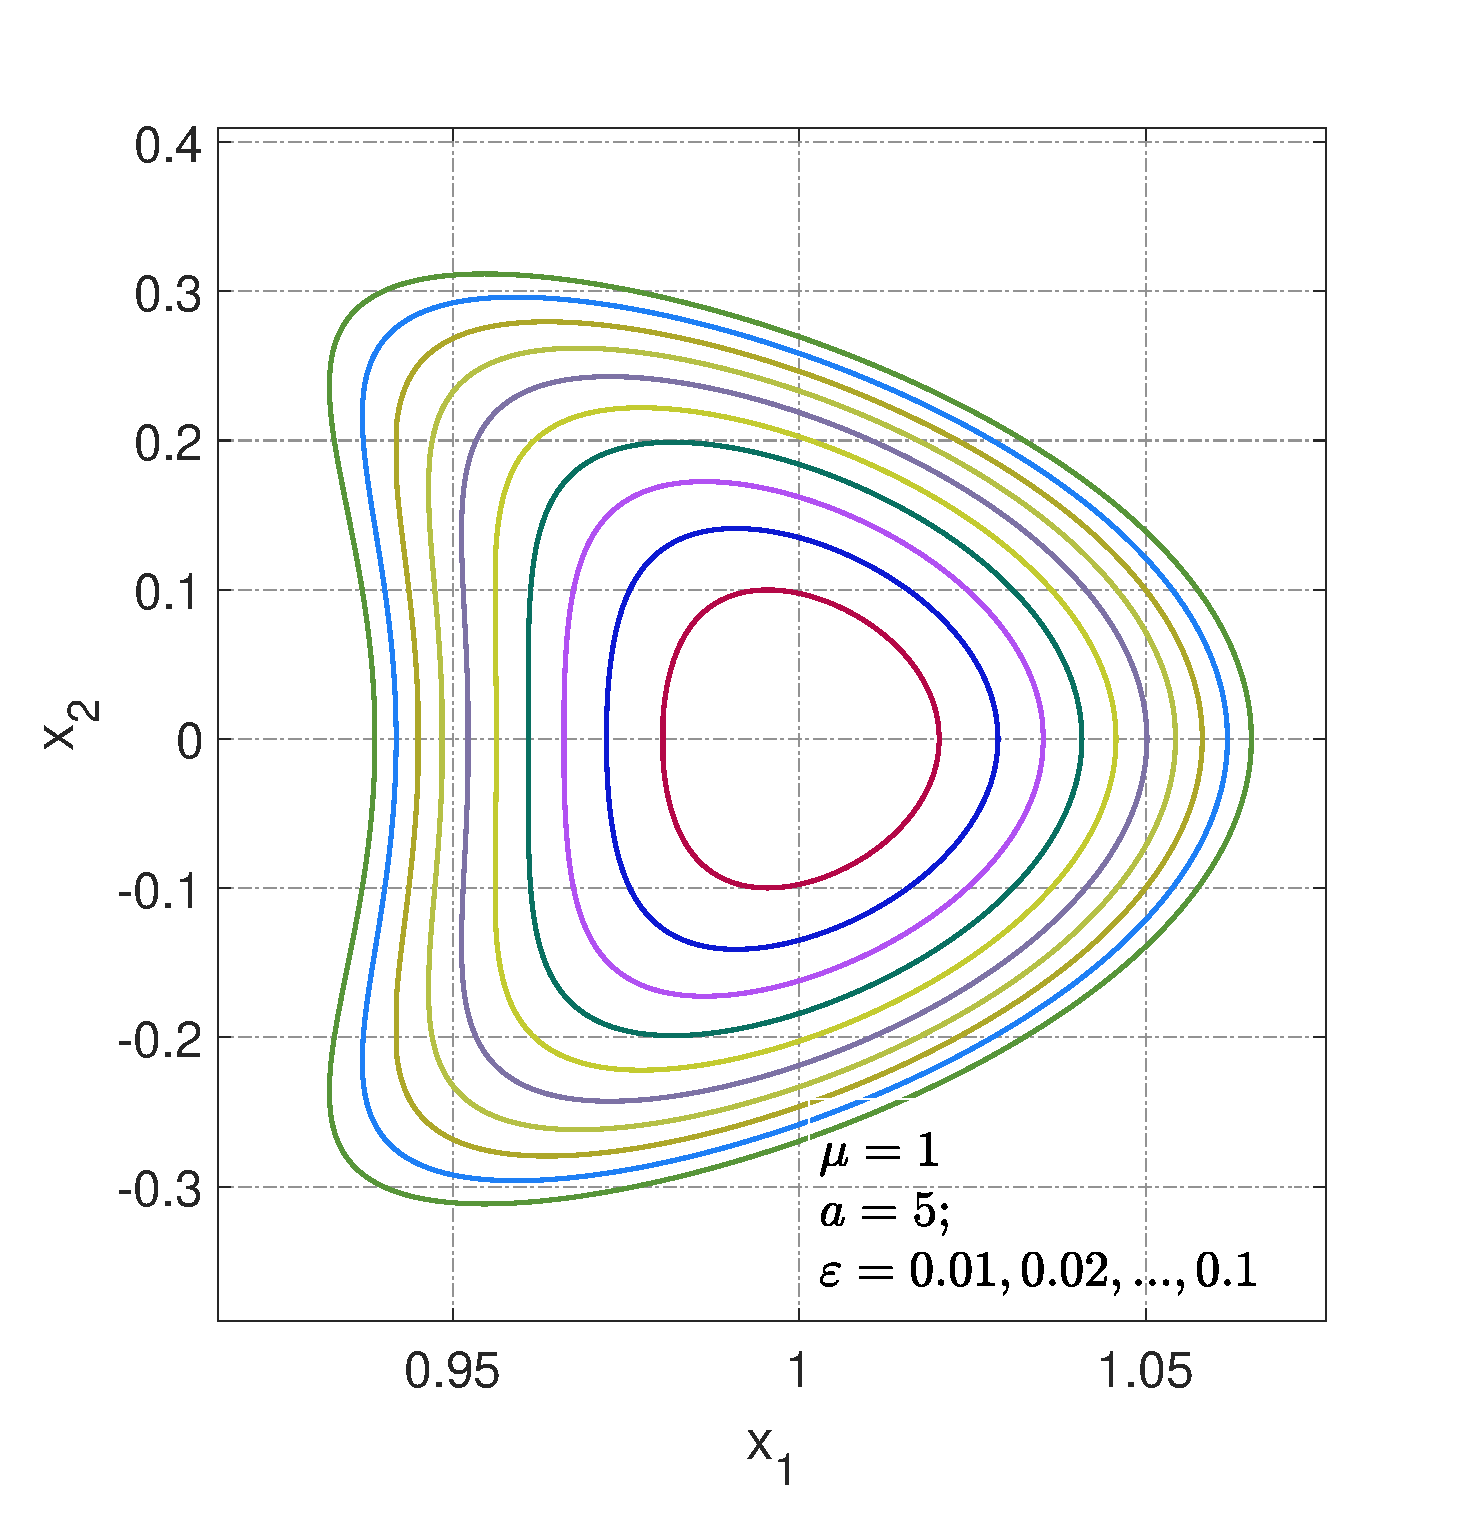
\includegraphics[width=1.05\linewidth]{images/figb11.eps}}
	 \end{minipage}
	 \hfill
	 \begin{minipage}[h]{0.5\linewidth}
		 \center{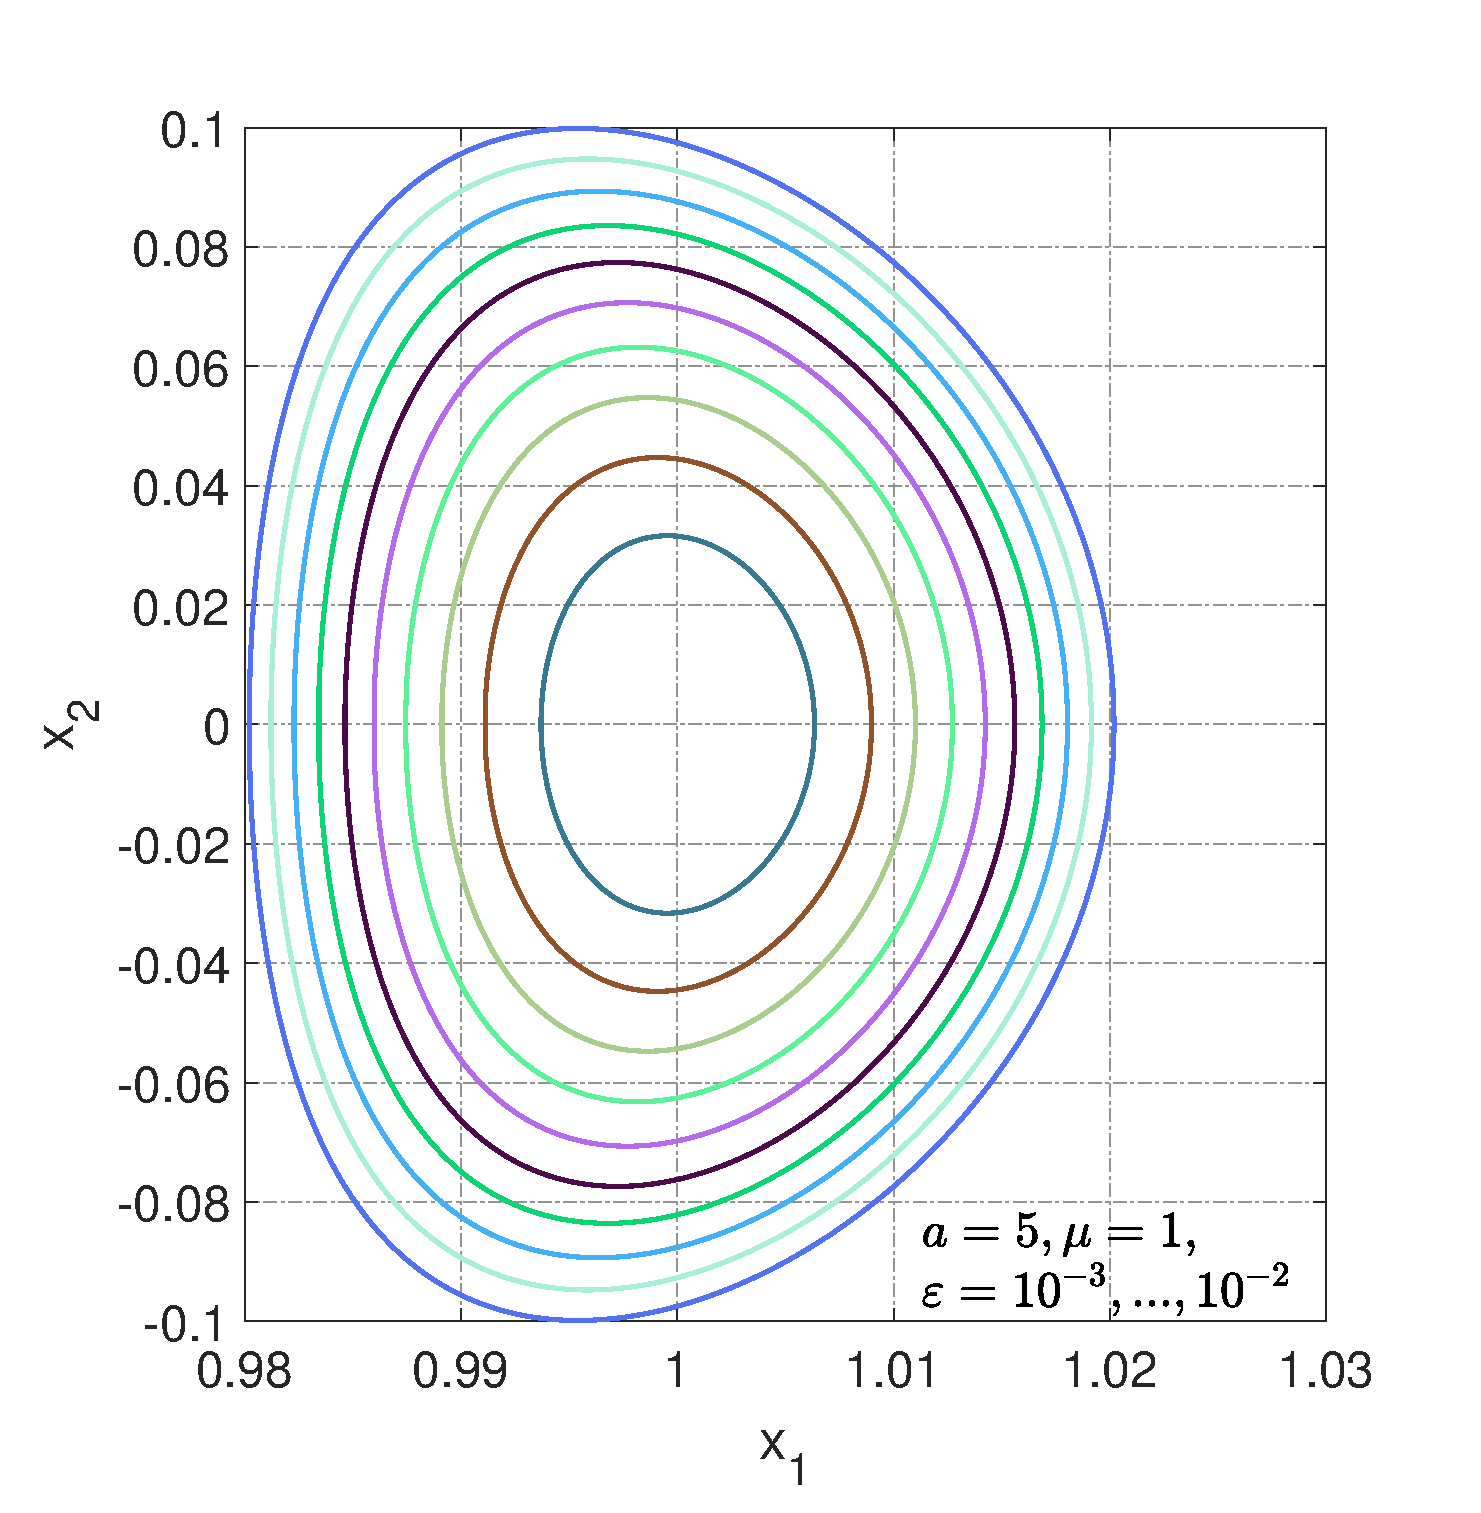
\includegraphics[width=1.05\linewidth]{images/figb21.eps}}
	 \end{minipage}
	 \caption{Множества достижимости билинейной системы}
	 \label{fig:fig31}
 \end{figure}
 
 
 
 
 Для описания области достижимости системы \eqref{brokett} введем вспомогательную линейную систему
 \begin{equation}\label{linearbrokett}
	 \left[ {\begin{array}{*{20}{c}}
			 {{{\dot y}_1}}\\
			 {{{\dot y}_2}}
	 \end{array}} \right] = \left[ {\begin{array}{*{20}{c}}
			 0&{ - 1}\\
			 1&0
	 \end{array}} \right]\left[ {\begin{array}{*{20}{c}}
			 {{u_1}}\\
			 {{u_2}}
	 \end{array}} \right],
 \end{equation}
 множество достижимости которой является эллипсом $ G(t_1) = \left\lbrace y | y^T \left( B B^T\right)  ^{-1} y \leq \mu^2 \right\rbrace  $, где 
 \begin{equation*}
	 B = \left[ {\begin{array}{*{20}{c}}
			 0&{ - 1}\\
			 1&0
	 \end{array}} \right].
 \end{equation*}
 
 Таким образом, множество достижимости системы \eqref{brokett} может быть получено путем нелинейного преобразования множества достижимости $ G(t_1) $ линейной системы \eqref{linearbrokett}. На рисунке  \ref{fig:fig31} показаны множества достижимости для различных $ \varepsilon $.
 
 
 \begin{equation*}
	 \begin{array}{l}
		 r({t_1}) = {e^{ \frac{1}{a} y_1}}\\
		 \varphi ({t_1}) =  y_2. 
	 \end{array}
 \end{equation*}
 % ссылка на тарасьева
 \paragraph{Машина Дубинса.} 
 Рассмотрим систему 
 \begin{equation}\label{system6}
	 \begin{array}{*{20}{c}}
		 {\left\{ {\begin{array}{*{20}{l}}
					 {{{\dot x}_1} = \cos {x_3}}\\
					 {{{\dot x}_2} = \sin {x_3}}\\
					 {{{\dot x}_3} = u}
			 \end{array}} \right.}&{{x_1}\left( 0 \right) = {x_2}\left( 0 \right) = {x_3}\left( 0 \right) = 0}
	 \end{array}
 \end{equation}
 на отрезке $ \left[0;\varepsilon \right] $, где $ \varepsilon > 0 $. Ограничения на $ u\left(t \right) $ заданы неравенством 
 \begin{equation}\label{constraints*}
	 \int_{0}^{\vartheta} u^2(\tau) d\tau \leqslant \mu^2.
 \end{equation}
 
 При $  u_1(t) \equiv 0 $ получаем траекторию $ x_1(t) = t, \ x_2(t) = x_3(t) \equiv 0 $. Как и в предыдущем примере, линеаризуем систему вдоль траектории, порожденной нулевым управлением
 \begin{equation}\label{system6l}
	 \left[ {\begin{array}{*{20}{c}}
			 {{{\dot x}_1}}\\
			 {{{\dot x}_2}}\\
			 {{{\dot x}_3}}
	 \end{array}} \right] = \varepsilon \underbrace {\left[ {\begin{array}{*{20}{c}}
				 0&0&0\\
				 0&0&1\\
				 0&0&0
		 \end{array}} \right]}_A\left[ {\begin{array}{*{20}{c}}
			 {{x_1}}\\
			 {{x_2}}
	 \end{array}} \right] + \underbrace {\left[ {\begin{array}{*{20}{c}}
				 0\\
				 0\\
				 1
		 \end{array}} \right]}_Bu ,
 \end{equation}
 \begin{figure}[h]
	 \centering
	 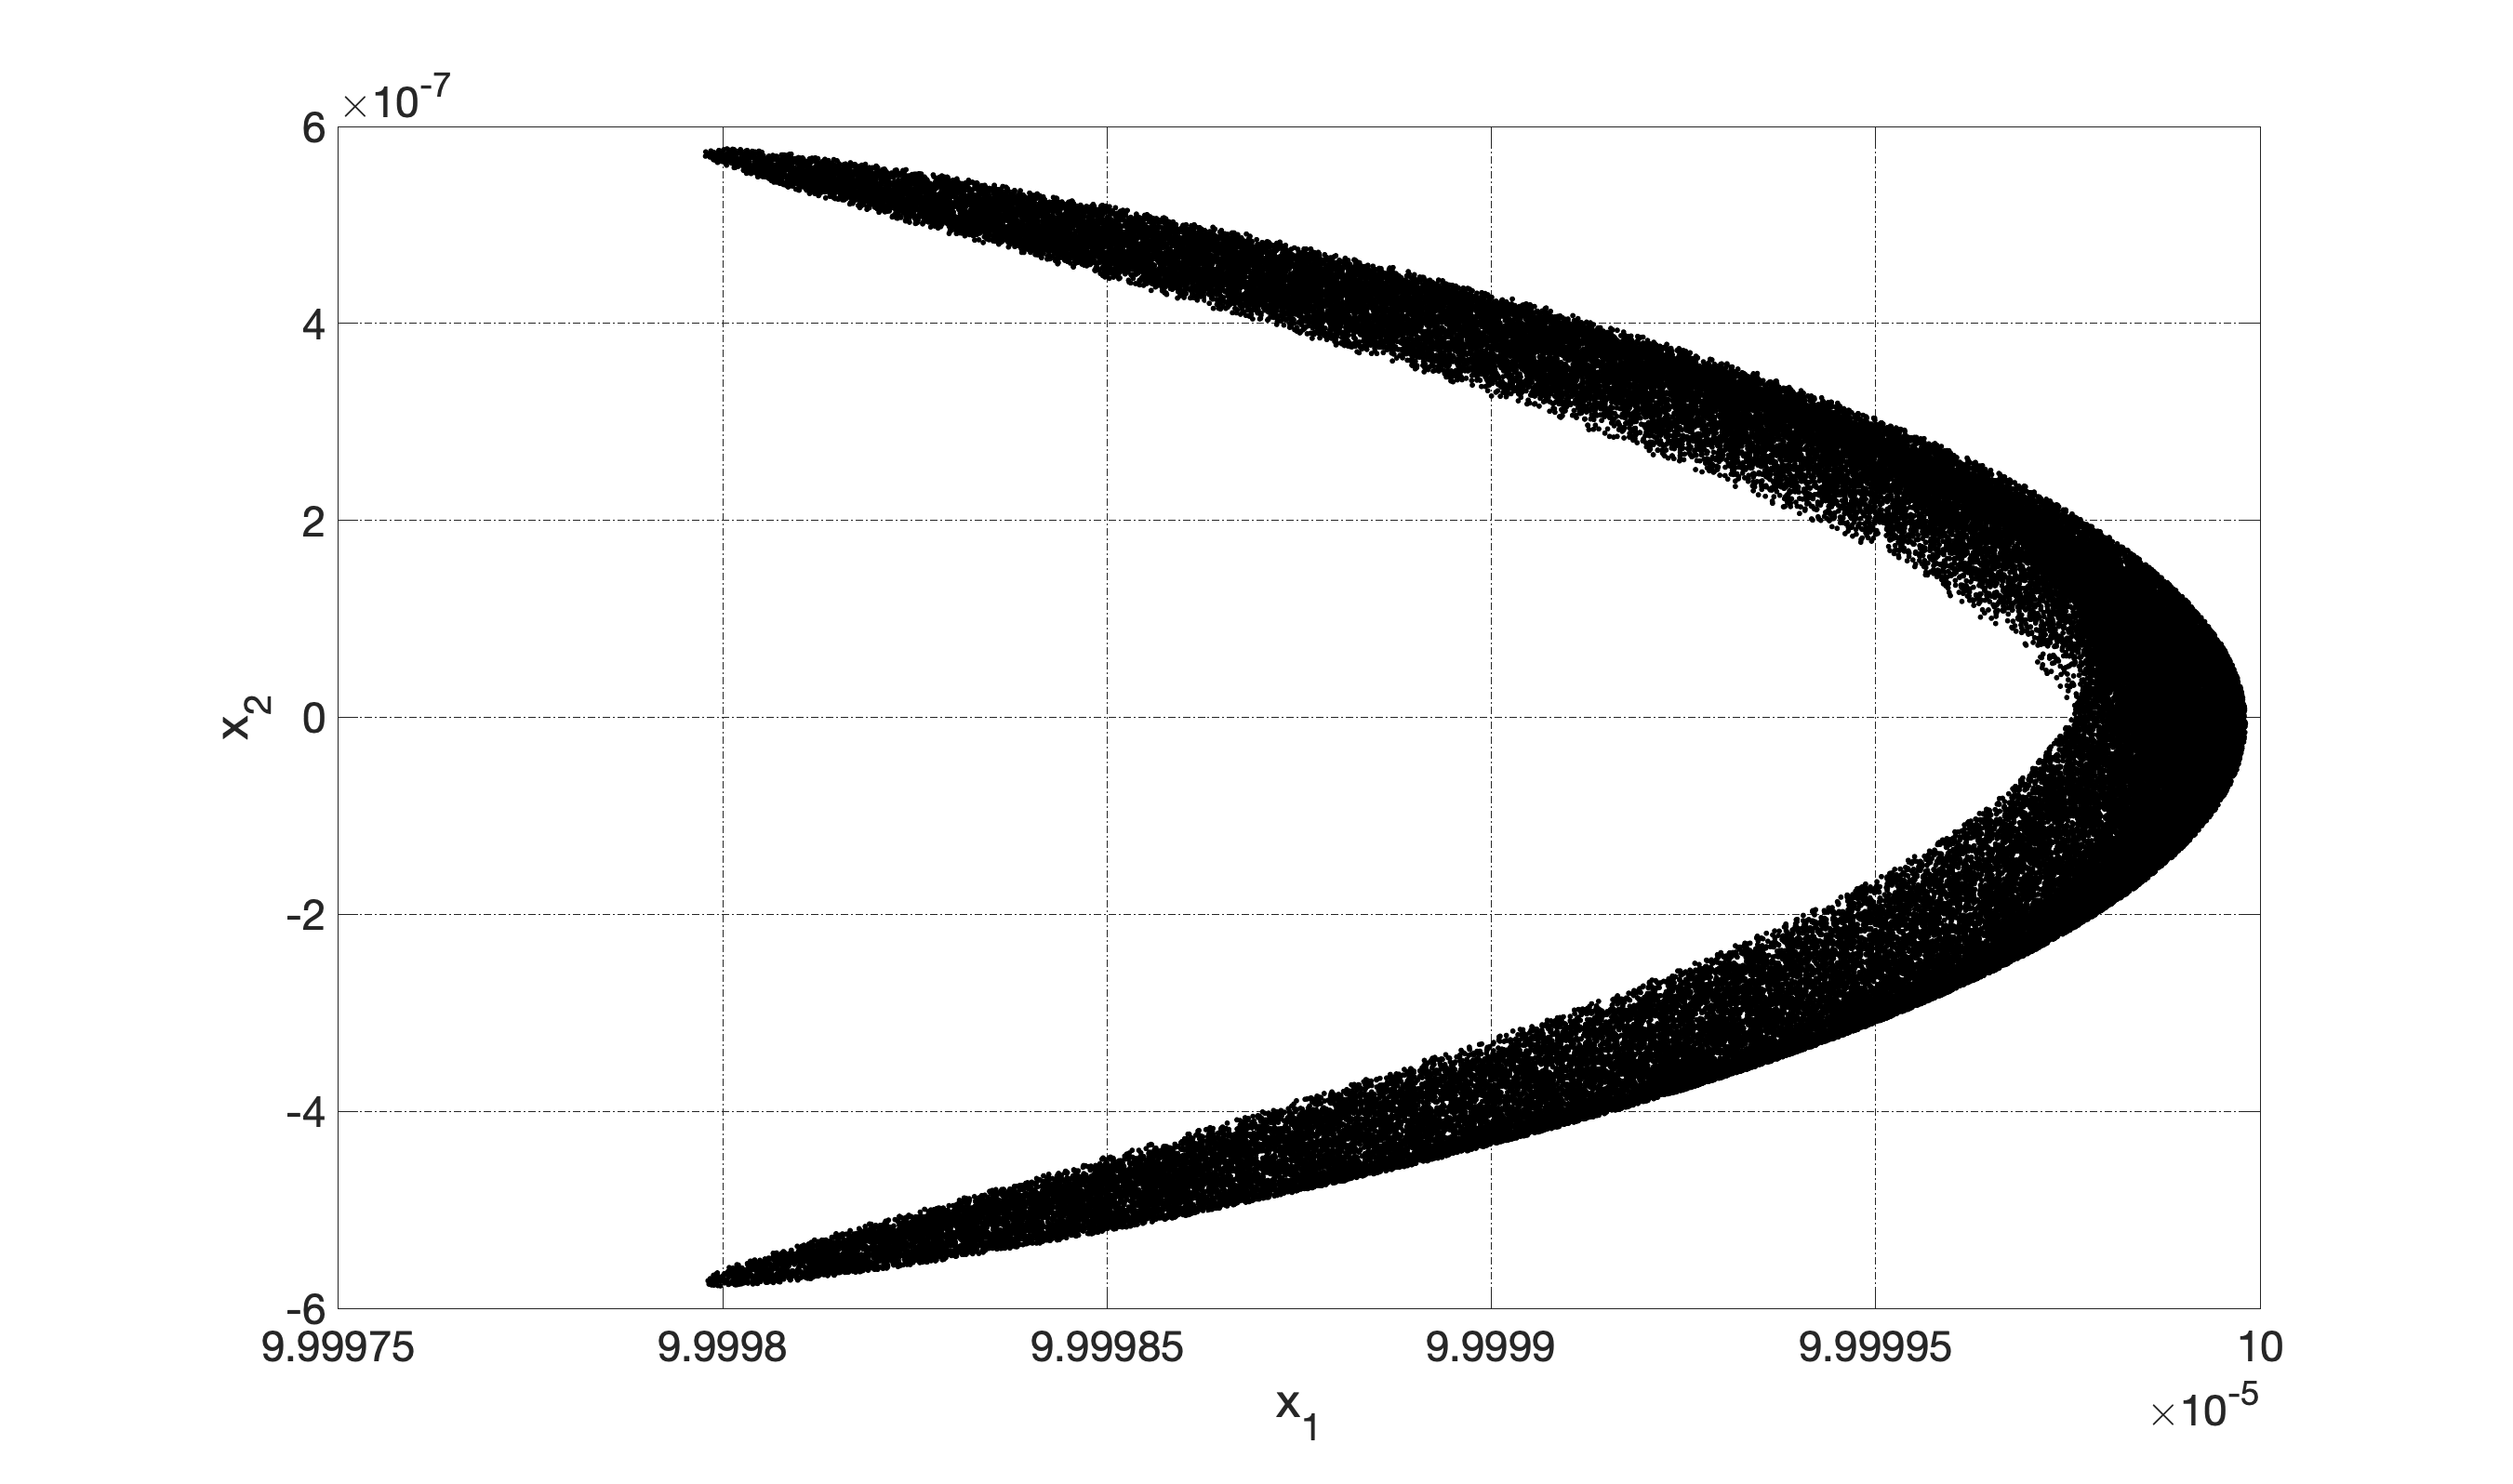
\includegraphics[width=1\linewidth]{images/fig52.eps}
	 \caption{Множество достижимости машины Дубинса для $\varepsilon = 10^{-4}, \mu = 1$.}
	 \label{fig:fig3}
 \end{figure}
 Очевидно, что система \eqref{system6l} неуправляема по 1-ой координате, следовательно, ее граммиан управляемости содержит нулевое собственное число, из-за которого условие \eqref{cond} не выполняется. Следовательно, система \eqref{system6} может иметь невыпуклые множества достижимости на малых промежутках времени.
 
 Воспользовавшись численным алгоритмом построения множеств достижимости систем с интегральными ограничениями \cite{GusevZykov2018} построим множество достижимости \eqref{system6} для $ \mu = 1  $ и $ \varepsilon = 0.0001  $ c. 
 
 Моделирование показывает, что множество достижимости <<машины Дубинса>> невыпукло для достаточно малых $ \varepsilon $; это можно показать и теоретически, но строгое доказательство невыпуклости выходит за рамки этого раздела.
 
\end{document}